\documentclass[paper=a4, fontsize=11pt, toc=listof, toc=bib, open=any, twoside=false, onehalfspacing, titlepage=firstiscover, headings=normal]{scrbook}

% Packages, layout and theorem environments. Notation macros live in notation.tex.

\setcounter{tocdepth}{\subsectiontocdepth}

\usepackage[utf8]{inputenc}
\usepackage[bottom=4cm, inner=3cm, outer=3cm]{geometry}
\usepackage[headsepline]{scrlayer-scrpage}
\usepackage[backend=biber, citestyle=authoryear-comp, bibstyle=authoryear-comp, mergedate=compact, natbib=true, sorting=nyt, sortcites=true]{biblatex}
\usepackage{setspace}
\usepackage{graphicx}
\usepackage{booktabs}
\usepackage{csquotes}
\usepackage{amsmath, amsthm, amssymb}
\usepackage{hyperref}

\addbibresource{references.bib}
\graphicspath{{figures/}}

\setkomafont{pageheadfoot}{\scshape}
\pagestyle{scrheadings}
\addtokomafont{disposition}{\rmfamily}

% Theorem environments, one shared counter per chapter (Lemma 3.1, Theorem 3.2, ...)
\theoremstyle{plain}
\newtheorem{theorem}{Theorem}[chapter]
\newtheorem{lemma}[theorem]{Lemma}
\newtheorem{proposition}[theorem]{Proposition}
\newtheorem{corollary}[theorem]{Corollary}
\newtheorem{conjecture}[theorem]{Conjecture}
\theoremstyle{definition}
\newtheorem{definition}[theorem]{Definition}
\newtheorem{example}[theorem]{Example}
\theoremstyle{remark}
\newtheorem{remark}[theorem]{Remark}

% Notation. Every symbol that appears in more than one chapter is defined here once.
% Conventions: theta (not tau) for dispersion, eta for private noise,
% q = m mod n is the REMAINDER, r = floor(m/n) the number of full rounds.

% Sets, allocations, valuations
\newcommand{\Agents}{N}
\newcommand{\Goods}{M}
\newcommand{\Alloc}{A}
\newcommand{\Allocs}{\Pi_n(\Goods)}

% Target quantity
\newcommand{\astar}{\alpha^{*}}
\newcommand{\aij}{\alpha_{ij}}

% Survival function and its estimator
\newcommand{\Surv}{S_X}
\newcommand{\Survhat}{\hat{S}_X}

% Sampling model
\newcommand{\Zig}{Z_{ig}}
\newcommand{\Wg}{W_g}
\newcommand{\etaig}{\eta_{ig}}

% Operators
\DeclareMathOperator{\Corr}{Corr}
\DeclareMathOperator{\Var}{Var}
\DeclareMathOperator*{\argmax}{arg\,max}


% Compile only selected chapters, e.g. the five correction pages for Matthias.
% Page numbers and references stay consistent. Comment out to compile everything.
%\includeonly{chapters/03_model}

\begin{document}

\frontmatter
% Title page, \input from main.tex
\begin{titlepage}
	\begin{center}
		
\includegraphics[width=.4\textwidth]{KITLogo_RGB.pdf}\\
		
		\vspace*{2cm}
		\Huge{\scshape How Often Does Round Robin Achieve EFX? A Simulation-Based Average-Case Analysis} % hier den Titel der Thesis eintragen/insert title here
		
		\vspace*{\fill}
		\Large{Bachelor's Thesis\\by} % Typ der Thesis hier eintragen/specify type of thesis here
		
		\vspace*{1cm}
		\LARGE{\scshape Francisco Waggershauser\\} % hier Namen eintragen/your name here
		
		\vspace*{0.5cm}
		\normalsize{Matriculation Number: 2474586\\ % hier Matrikelnummer eintragen/your matr. number here
		Course of Studies: Industrial Engineering \& Management} % hier Studiengang eintragen/your study program here
		
		\vspace*{1cm}
		\Large{at the\\}
		\vspace*{0.5cm}
		\normalsize{
			Department of Economics and Management\\
			Institute of Economics (ECON)\\
			Chair of Economic Theory}
	\end{center}
	\vspace*{\fill}
	\small
	\begin{tabular}[ht]{l c l}
			Examiner: & \hfill  & Prof. Dr. Clemens Puppe\\
			Co-Examiner: & \hfill & Dr. Hannes Rau\\ % hier den Zweitprüfer eintragen/co-examiner here
			Supervisor: & \hfill  & Matthias Ammann\\
			Submission Date: & \hfill & xx/xx/202x % Abgabedatum hier eintragen/hand-in date here
	\end{tabular}
\end{titlepage}


\newgeometry{bottom=4.5cm, left=2cm, right=2.5cm}

% Abstract, \input from main.tex
\chapter*{Abstract}
%% FUNCTION: States the question, the method, the main findings and the recommendation in one
%% paragraph.

Round Robin, in which people take turns picking their favourite remaining good, is a fair
division procedure that can be carried out by hand. It always guarantees envy-freeness up to one
good (EF1), but it offers no guarantee, not even an approximate one, for the stronger notion of
envy-freeness up to any good (EFX). We therefore ask how often Round Robin achieves EFX in the
average case and under which conditions it is a good heuristic for EFX. We simulate
$20{,}000$ instances for each combination of two to five agents, up to four goods per agent and
lognormal values with five levels of agreement and six levels of dispersion, and vary one
condition at a time around a reference cell. In the reference cell with four agents and twelve
goods, Round Robin achieves EFX in $29\%$ of the instances. It achieves EFX more often when agents
agree little, when values are similar and the number of goods is divisible by the number of
agents, and when every agent receives more goods; it achieves EFX less often, and misses it by
more, when agents agree strongly, values differ greatly or more agents take part. We prove that
Round Robin is always EFX when every agent receives at most two goods and all favourite goods
differ, and that it is never EFX under identical valuations when the number of goods is not
divisible by the number of agents. Compared with a random allocation of equal bundle sizes,
Round Robin is far ahead unless agents agree strongly, and reversing the order of the last round
removes its systematic failure under identical valuations. A decision table summarises when Round
Robin can be relied on.


\tableofcontents
\listoftables
\listoffigures

\mainmatter
\doublespacing

\chapter{Introduction}\label{ch:intro}
%% FUNCTION: Motivates the question and states what the thesis contributes: practice first
%% (round robin works by hand), then theory (EF1 guaranteed, EFX existence open from four agents
%% on, no approximation guarantee for EFX), then the gap, the research question, the
%% contributions and a roadmap. No mathematics in this chapter (chair writing guide).

When heirs divide an estate, flatmates split the furniture of a shared flat or children share a
box of toys, a common procedure is to take turns: everyone picks the item they like best among
those that remain, in a fixed order, round after round. This procedure is called Round Robin. It
needs no computer, no money and no announcement of how much anyone values each item; everyone
only has to make a choice when it is their turn. Variants of it are used in practice, for instance
in a draft at Harvard Business School that allocated courses to students and reversed the order
of choosing in every round \parencite[p.~1065]{budish2011}.

Procedures that do better are available, but they cannot be carried out by hand. A local search
procedure, for instance, finds a fair allocation in the sense studied here in every instance that
has been tested, but it does so by moving goods between bundles thousands of times
\parencite{branzei2025}. For a family at a kitchen table, the realistic alternative to Round Robin
is therefore not the best possible allocation, but dividing the goods somehow. The question is
whether taking turns is good enough.

What counts as fair is a question of theory. The most demanding standard, that nobody prefers
another person's share to their own, often cannot be met when goods are indivisible: with one
painting and two heirs, one of them is left without it. The literature therefore uses weaker
standards. Round Robin always meets a weak one: if someone prefers another person's share, this
preference disappears once a single good, the one they like best, is removed from the other
share \parencite{caragiannis2019,amanatidis2023survey}. This standard is called envy-freeness up
to one good (EF1). A stronger standard requires that the
preference disappears after removing \emph{any} single good from the other share, even the one
they like least; it is called envy-freeness up to any good (EFX). Whether an allocation meeting this stronger standard always exists is one of the
main open questions of the field for four or more people
\parencite[Open Problem~2]{amanatidis2023survey}. Round Robin offers no guarantee for it, not even
an approximate one: in some situations, its allocation misses the stronger standard by an
arbitrarily large factor (Chapter~\ref{ch:background}). A guarantee for the worst case therefore
says nothing useful, and only the typical case can tell whether Round Robin is a good way to reach
the stronger standard.

Existing studies of the typical case of such turn-taking procedures concern other goals. Some
ask which order of turns maximises the expected total or minimum satisfaction
\parencite{bouveret2011,kalinowski2013}. Others prove that, as the number of people grows and their
valuations are independent, Round Robin even reaches the most demanding standard once there are
enough goods, and that a variant which reverses the order of the last round reaches the stronger
standard with high probability \parencite{manurangsi2021}. These results are asymptotic and assume
that people value goods independently of each other. For a few people, for people who largely
agree on what is valuable, and for the question of how far Round Robin misses the stronger standard
when it fails, we found no analysis. \textcite[p.~11]{branzei2025} remarks that Round Robin often
fails it, especially when valuations are correlated, but does not quantify this.

This thesis asks: \emph{how often does Round Robin achieve EFX, and under which conditions is it
therefore a good heuristic for EFX?} We answer the question by simulation. We
vary five conditions one at a time around a common reference case: how much the people agree,
how far apart the values of the goods lie, how many goods each person receives, whether the goods
can be divided evenly, and how many people take part. For each combination, we draw
20{,}000 situations and measure both how often Round Robin succeeds and how far it misses when
it fails.

The thesis makes three contributions. First, it measures how often Round Robin reaches the
stronger standard and how far it misses it, for two to five people and for valuations that range
from independent to identical. Second, it proves three simple statements that delimit these
measurements: Round Robin always succeeds when everyone receives at most two goods and nobody
shares a favourite good; it always fails when everyone ranks the goods identically and the goods
cannot be divided evenly; and when all goods are worth almost the same and can be divided evenly,
it almost always succeeds. Third, it compares Round Robin with dividing the goods at random and
with reversing the last round, and it collects the results in a table that tells people who divide
goods by hand when to rely on Round Robin.

Chapter~\ref{ch:background} defines the fairness standards and explains why Round Robin meets the
weaker but not the stronger one. Chapter~\ref{ch:model} describes the simulation.
Chapter~\ref{ch:results} presents the results one condition at a time, and
Chapter~\ref{ch:random} compares Round Robin with random allocation and with reversing the last
round. Chapter~\ref{ch:discussion} discusses limitations and open questions, and
Chapter~\ref{ch:conclusion} concludes with the decision table.

\chapter{Round Robin, EF1 and EFX}\label{ch:background}

%% FUNCTION: This chapter provides the concepts that every later result relies on and explains why
%% round robin achieves EF1 but not necessarily EFX.



\section{Setting and Notation}\label{sec:setting}
%% FUNCTION: Introduces agents, goods, additive valuations, allocations, picking sequences and
%% Round Robin, together with the number of full rounds and the remainder of goods. All later
%% chapters use this notation.

We consider a set of agents $N = \{1,\dots,n\}$ as well as a set of indivisible goods $M = \{g_1,\dots,g_m\}$. Each agent has an additive \textit{valuation function} $v_i(S)$, where $S \subseteq M$ and $v_i(S)=\sum_{g\in S} v_i(g)$, with $v_i(g) \geq 0$. The model (see Chapter~\ref{ch:model}) generates strictly positive, continuous values. 

An \textit{allocation} $A = (A_1,\dots,A_n)$ is a tuple of subsets of $M$ ($A_i \subseteq M$), so that every agent $i \in N$ gets a \textit{bundle} assigned. The bundles are pairwise disjoint ($A_i \cap A_j = \emptyset$ for $i \neq j$), and complete ($\bigcup_{i \in N} A_i = M$).

We define a \textit{picking sequence} following \textcite{bouveret2011} as a sequence $(\sigma_1,\dots,\sigma_m) \in N^m$. In turn $k$ agent $\sigma_k$ chooses the good with the highest $v_{\sigma_k}(g)$ from the remaining goods. Ties are broken by a fixed rule; under continuous valuations they occur with probability zero (Chapter~\ref{ch:model}).

The central picking sequence of this work is Round Robin. It repeats the order
$1,2,\dots,n$ until $m$ turns are reached. Round $t$ consists of the turns $(t-1)n+1$ to $tn$. The last round can be incomplete. The good that agent $i$ takes in round $t$ is $i_t$. The bundle of agent $i$ is $A_i=\{i_1,\dots,i_{|A_i|}\}$.

Following \textcite{manurangsi2021}, we define two variables $r$ and $q$. Here, $r$ is the number of \textit{full rounds} defined as $r = \lfloor \frac{m}{n} \rfloor$ and $q = m - nr$ which is the remainder of goods in the last round. If $q=0$, then $m$ is divisible by $n$ and there is no incomplete round. Applied to the Round Robin algorithm, that means that the agents $1,\dots,q$ get $r+1$ goods and the other remaining agents $r$ goods.

\begin{example}
Let $n=3$, $m=7$, thus $r = \lfloor \frac{7}{3}\rfloor =2$ and $q = 1$: the sequence of Round Robin is 1231231. The bundle sizes for the agents are 3, 2, 2.
\end{example}


\section{Fairness Notions}\label{sec:notions}
%% FUNCTION: Defines envy freeness, EF1, EFX and its approximate version, the alpha-EFX ratio used
%% as the target quantity, each attributed to its source. The section shows how the notions relate
%% to each other.

\paragraph{Envy-freeness (EF).}
The fair division literature has developed various fairness concepts over time. The goal is to find a \textit{fair allocation} that fulfils such a concept. One of the most established fairness notions is \textit{envy-freeness} (EF). Following \textcite[Def.~1]{amanatidis2023survey}, an allocation $A$ is EF if $v_i(A_i)\geq v_i(A_j)$ for all $i,j\in N$. That means, every agent values their own bundle at least as much as any other bundle. For indivisible goods, EF turns out to be a very strict notion that often cannot be achieved. The simple example of two agents ($n=2$) and a single good ($M=\{g\}$) shows this: in every allocation, the agent without the good envies the other agent, as long as they value the good positively.

\paragraph{Envy-freeness up to one good (EF1).}
Consequently, different relaxations of envy-freeness began to emerge. One of the most established relaxations is \textit{envy-freeness up to one good} (EF1). The idea goes back to \textcite{lipton2004}, who bound the envy between two agents by the value of a single good, and \textcite[Def.~3]{budish2011} formalised it as ``envy bounded by a single good''. An allocation $A$ is EF1 if for all $i,j\in N$ with $A_j\neq\emptyset$ there exists a good $g\in A_j$ with $v_i(A_i)\geq v_i(A_j\setminus\{g\})$. Since removing the good that $i$ values most lowers $v_i(A_j)$ the most, this is equivalent to
\[
  v_i(A_i)\;\geq\; v_i(A_j)-\max_{g\in A_j} v_i(g).
\]
Hence, agent $i$ may still envy agent $j$, but the envy disappears once the good in $A_j$ that $i$ values most is removed. An EF1 allocation always exists: the envy-cycle elimination algorithm of \textcite[Thm.~2.1]{lipton2004} computes one in polynomial time. Section~\ref{sec:rrEF1} shows that Round Robin also always returns an EF1 allocation.

\paragraph{Envy-freeness up to any good (EFX).}
EF1 can always be achieved, but it is a relatively weak fairness notion: the envy only has to vanish after removing the good the envious agent likes most. The next major refinement is \textit{envy-freeness up to any good} (EFX), introduced by \textcite[Def.~4.5]{caragiannis2019}. An allocation $A$ is EFX if $v_i(A_i)\geq v_i(A_j\setminus\{g\})$ for all $i,j\in N$ and all $g\in A_j$ with $v_i(g)>0$. The condition is hardest to satisfy for the good that $i$ values least, so whenever $A_j$ contains a good that $i$ values positively, this is equivalent to
\[
  v_i(A_i)\;\geq\; v_i(A_j)-\min\{v_i(g) : g\in A_j,\ v_i(g)>0\}.
\]
In this case, agent $i$ may still envy agent $j$, but the envy disappears after removing \emph{any} good from $A_j$, in particular the one that $i$ values least. The standard formulation in \textcite[Def.~4]{amanatidis2023survey} drops the condition $v_i(g)>0$. The two versions differ only when some goods have value zero. Since our model generates strictly positive values (Chapter~\ref{ch:model}), they coincide in this thesis.

\paragraph{Hierarchy.}
EFX is one of the central notions of current research in fair division \parencite{amanatidis2023survey}. All of these fairness notions are logically connected: $\mathrm{EF}\Rightarrow\mathrm{EFX}\Rightarrow\mathrm{EF1}$, but not the other way around \parencite[p.~8]{amanatidis2023survey}. Whether an EFX allocation always exists is open for four or more agents (Section~\ref{sec:existence}).

If every bundle contains at most one good, every allocation is EFX, because removing that good leaves an empty bundle of value zero. For $m\leq n$, Round Robin gives every agent at most one good, so EFX holds trivially. We therefore assume $m>n$ from now on.

\paragraph{$\alpha$-EFX and our target quantity.}
Since the existence of exact EFX allocations is open in general, a second line of research relaxes EFX by a multiplicative factor: an agent only has to receive a fixed share $\alpha$ of the value that EFX would guarantee. Following \textcite[Def.~8]{amanatidis2023survey}, an allocation $A$ is \textit{$\alpha$-EFX} for $\alpha\in(0,1]$ if
\[
  v_i(A_i)\;\geq\;\alpha\cdot v_i(A_j\setminus\{g\})
\]
for all $i,j\in N$ and all $g\in A_j$ with $v_i(g)>0$. Earlier versions of this notion appear as $c$-EFX in \textcite[Def.~2.5]{plaut2020} and as $\alpha$-EFX in \textcite[Def.~2.2]{amanatidis2018comparing}.

For a pair of agents $i\neq j$, we measure how close the allocation comes to EFX by the largest $\alpha$ for which this inequality holds for every such $g$. Again, the binding good is the one that $i$ values least, which gives
\[
  \aij \;=\; \frac{v_i(A_i)}{v_i(A_j)-\min\{v_i(g) : g\in A_j,\ v_i(g)>0\}}.
\]
Taking the worst pair over all comparisons between agents gives our target quantity
\[
  \astar \;=\; \min\Big\{1,\ \min_{i\neq j}\aij\Big\}.
\]
By construction, $\astar=1$ if and only if $A$ is EFX. It is important to note that $\aij$ can be larger than $1$, but $\astar$ is capped at $1$. Furthermore, if $A_j$ contains only one good that $i$ values positively, the denominator is zero: removing this good leaves nothing that $i$ values, so EFX holds trivially for this pair and $\aij$ is not defined. Such pairs do not enter the minimum (Chapter~\ref{ch:model}). For example, $\astar=0.8$ means that the worst-off agent values their own bundle at $80\%$ of what EFX would require in the comparison that binds most.

This relaxation matters for Round Robin. An EF1 allocation is not necessarily $\alpha$-EFX for any $\alpha\in(0,1]$ \parencite[Prop.~3.1]{amanatidis2018comparing}. Section~\ref{sec:rrEF1} shows that this also holds for the allocations that Round Robin produces, which is why we study $\astar$ in the average case.


\section{Why Round Robin Is EF1 but Not Approximately EFX}\label{sec:rrEF1}
%% FUNCTION: Restates the known argument that round robin is EF1. A worst case example shows that
%% round robin has no constant approximation guarantee for EFX, which motivates the average case
%% question of the thesis.

Round Robin always returns an EF1 allocation \parencite[p.~12:7]{caragiannis2019}. The argument
is short, and it shows where EFX can fail, so we restate it following
\textcite[Thm.~1]{amanatidis2023survey}. Recall that $i_t$ denotes the good that agent $i$ picks
in round $t$.

\begin{proposition}\label{prop:rrEF1}
Let $A$ be the Round Robin allocation. For agents $i<j$, we have $v_i(A_i)\geq v_i(A_j)$. For
agents $i>j$, we have $v_i(A_i)\geq v_i(A_j)-v_i(j_1)$. In particular, $A$ is EF1.
\end{proposition}

\begin{proof}
Let $i<j$. In every round, agent $i$ picks before agent $j$, so the good $j_t$ was still available
when $i$ picked $i_t$, and $v_i(i_t)\geq v_i(j_t)$. Since $|A_i|\geq|A_j|$, summing over the rounds
gives $v_i(A_i)\geq v_i(A_j)$. Let $i>j$. Now $j$ picks before $i$ in every round, but the good
$j_{t+1}$ that $j$ picks in the next round was still available when $i$ picked $i_t$, so
$v_i(i_t)\geq v_i(j_{t+1})$. Since $|A_i|\geq|A_j|-1$, summing over the rounds gives
$v_i(A_i)\geq v_i(A_j\setminus\{j_1\})$.
\end{proof}

Envy can therefore only point from an agent who picks later to an agent who picks earlier, and it
disappears once the earlier agent's first good is removed. EFX, in contrast, requires that the
envy disappears after removing the earlier agent's \emph{least} valuable good. Nothing in the
argument controls this, and the following example shows that the shortfall can be arbitrarily large.

\begin{example}\label{ex:witness}
Let $n=2$, $m=4$ and $0<\delta<1/3$, with values
\[
  v_1=(10,\,1,\,9,\,1),\qquad v_2=(1,\,3\delta,\,2\delta,\,\delta)
\]
for the goods $g_1,\dots,g_4$. Round Robin with the sequence $(1,2,1,2)$ proceeds as follows:
agent $1$ takes $g_1$, agent $2$ takes $g_2$, agent $1$ takes $g_3$, and agent $2$ takes $g_4$.
Hence $A_1=\{g_1,g_3\}$ and $A_2=\{g_2,g_4\}$. Agent $2$ values their own bundle at $4\delta$ and
agent $1$'s bundle at $1+2\delta$; removing the good in $A_1$ that agent $2$ values least, $g_3$,
leaves a value of $1$. Thus $\alpha_{21}=4\delta$. Agent $1$ does not envy agent $2$ at all
($\alpha_{12}=19$), so $\astar=4\delta$, which tends to $0$ as $\delta\to0$.
\end{example}

The allocation in the example is EF1, as Proposition~\ref{prop:rrEF1} guarantees, but for every
$\alpha\in(0,1]$ there is an instance in which it is not $\alpha$-EFX (proven). This is the Round
Robin counterpart of the general observation that an EF1 allocation need not be $\alpha$-EFX for
any $\alpha>0$ \parencite[Prop.~3.1]{amanatidis2018comparing}. In every single instance,
$\astar>0$, but no positive lower bound holds for all instances. A worst case analysis therefore
says nothing about how well Round Robin approximates EFX, and only the average case over a
distribution of instances is informative. This is the approach of this thesis.

\section{Does an EFX Allocation Exist?}\label{sec:existence}
%% FUNCTION: Summarises where the literature proves EFX existence and defines the region of our
%% design where it is open. For that region the section states explicitly that we assume
%% existence, and why. This tells the reader for every result whether a failure of round robin is
%% a failure of the mechanism or possibly of the problem itself.

When Round Robin fails to find an EFX allocation, this can mean two things: Round Robin missed an
EFX allocation that exists, or no EFX allocation exists at all. For additive valuations, whether
an EFX allocation always exists is open for four or more agents
\parencite[Open Problem~2]{amanatidis2023survey}. For several special cases, however, existence
is proven, and Table~\ref{tab:existence} lists those that cover cells of our design.

\begin{table}[ht]
  \centering
  \caption{Proven existence of EFX allocations and the cells of our design they cover.}
  \label{tab:existence}
  \small
  \begin{tabular}{p{4.6cm}p{4.4cm}p{4.2cm}}
    \toprule
    Condition & Source & Cells covered \\
    \midrule
    Two agents & \textcite{plaut2020} & all cells with $n=2$ \\
    Three agents, additive valuations & \textcite{chaudhury2024} & all cells with $n=3$ \\
    Identical valuations & \textcite{plaut2020}; alternative proof for additive valuations by \textcite[Prop.~1]{branzei2025} & all cells with $\rho=1$ \\
    At most three types of valuations & \textcite{hv2025} & only $\rho=1$ \\
    $m\leq n+2$, additive valuations & \textcite[Thm.~5.1]{amanatidis2020multiple} & $m=n+1,n+2$ \\
    $m\leq n+3$ & \textcite{mahara2024general} & $m=n+1,\dots,n+3$ \\
    \bottomrule
  \end{tabular}
\end{table}

In our design, existence is therefore open exactly for four or more agents, at least four goods
more than agents and less than full agreement: for $n=4$ from $m=8$ on and for $n=5$ from $m=9$
on, each with $\rho<1$. This region contains the reference cell. In this region, we
\textbf{assume} that an EFX allocation exists. Two observations support the assumption. Its
existence is widely conjectured \parencite[p.~2]{branzei2025}, and the local search of
\textcite{branzei2025} found an EFX allocation in every instance tested, including instances with
independent and with correlated values. None of these instances lies in our open region, the
closest being four agents with forty goods and independent values, so the assumption rests on the
direction of this evidence, not on a test of our cells. Under the assumption, every failure of
Round Robin is a failure of the mechanism. Outside the open region, this holds without any
assumption, and our results state in every section which case applies.

For approximate EFX, allocations that are $0.618$-EFX are known to exist and can be computed
efficiently \parencite[Thm.~4.4]{amanatidis2020multiple}; the best possible factor is open
\parencite[Open Problem~3]{amanatidis2023survey}. These algorithms are not meant to be carried
out by hand, which is the setting that motivates this thesis.

\chapter{Model and Simulation Design}\label{ch:model}
%% FUNCTION: Explains how we measure how often round robin achieves EFX, in the order in which the
%% simulation itself proceeds: a scenario (agents and goods), values for every agent and good, the
%% round robin allocation and its evaluation, and finally the design grid with the reference cell.
%% Random allocation and other picking sequences are introduced in Chapter 5, not here.

Our simulation proceeds in four steps, and this chapter follows them. A scenario fixes how many
agents share how many goods (Section~\ref{sec:scenario}). For every agent and good, we draw a
value (Section~\ref{sec:instances}). Round Robin allocates the goods, and we measure how close the
allocation comes to EFX (Section~\ref{sec:evaluation}). Repeating these steps many times for every
combination of parameters gives the design (Section~\ref{sec:design}).

\section{Scenario}\label{sec:scenario}

A scenario consists of $n$ agents and $m$ goods with $m>n$; for $m\leq n$, every allocation by
Round Robin is trivially EFX (Section~\ref{sec:notions}). Following
\textcite[p.~16]{manurangsi2021}, we write $m=rn+q$ with $r=\lfloor m/n\rfloor$ full rounds and a
remainder $0\leq q<n$. Under Round Robin, agents $1,\dots,q$ receive $r+1$ goods and the others
$r$ goods. For $q=0$, the number of goods is divisible by the number of agents, and every agent
receives the same number of goods.

The four quantities are linked by $m=rn+q$, so only some comparisons separate one effect from
another. Comparing different numbers of goods at a fixed number of agents changes $r$ or $q$ or
both, and comparing different numbers of agents at a fixed number of goods changes all of them.
We therefore never speak of an effect of $m$ alone. Instead, we compare
\begin{itemize}
  \item different $r$ at fixed $q$ (Section~\ref{sec:goods}),
  \item different $q$ at fixed $r$ (Section~\ref{sec:divisibility}), and
  \item different $n$ at fixed $r$ and $q$, that is, more agents with the same number of goods
  per agent (Section~\ref{sec:agents}).
\end{itemize}

\section{Values}\label{sec:instances}

We generate the value that an agent attributes to a good in two steps. In the first step, we
determine how the agents rank the goods. For every agent $i$ and good $g$, we draw a score $\Zig$
that consists of a common component $\Wg$, shared by all agents, and a private component $\etaig$,
which reflects the individual taste of agent $i$:
\[
  \Zig=\sqrt{\rho}\,\Wg+\sqrt{1-\rho}\,\etaig,\qquad \Wg,\etaig\sim\mathcal{N}(0,1).
\]
All $\Wg$ and $\etaig$ are mutually independent, and the parameter $\rho\in[0,1]$ sets the weight
of the common component. Two properties motivate this construction: $\Var(\Zig)=1$ for every
$\rho$, and $\Corr(\Zig,Z_{jg})=\rho$ for $i\neq j$. Thus, $\rho$ only influences how similarly the
agents rank the goods, not the distribution of a single score. For $\rho=0$, the rankings of
different agents are independent and uniformly distributed over all orderings of the goods,
whereas $\rho=1$ makes all rankings identical. These two endpoints coincide with the models
\textit{full independence} and \textit{full correlation} of \textcite[p.~74]{bouveret2011}. We call
$\rho$ the \textit{agreement}.

In the second step, we stretch $\Zig$ to obtain the value
\[
  v_i(g)=\exp(\theta\,\Zig),
\]
where $\theta>0$ controls how strongly the values are spread; we call it the
\textit{dispersion}. Each $v_i(g)$ is lognormally distributed, and this distribution does not
depend on $\rho$. The values are strictly positive and continuously distributed, so ties occur
with probability zero. As $\theta\to0$, all values tend to $1$, and every good is worth almost the
same. We chose the lognormal distribution because its values are positive and a single parameter
controls their spread. This is our own modelling choice. Similar models that combine a common and
an individual component appear in \textcite[p.~1406]{dickerson2014} and
\textcite[p.~8]{branzei2025}; in the latter, the parameter is a mixing weight rather than a
correlation.

We report both parameters on interpretable scales. Agreement is reported as the Spearman rank
correlation between the values of two agents over the goods,
\[
  \rho_S=\frac{6}{\pi}\arcsin\Big(\frac{\rho}{2}\Big),
\]
and dispersion as the Gini coefficient of the values of a single agent over the goods,
\[
  G=2\,\Phi\big(\theta/\sqrt{2}\big)-1,
\]
where $\Phi$ denotes the standard normal distribution function. Each scale reflects exactly one
parameter. Table~\ref{tab:axes} lists the levels used in this thesis. We report every Gini value
together with $\theta$ in parentheses.

\begin{table}[ht]
  \centering
  \caption{Parameter levels and their interpretable counterparts.}\label{tab:axes}
  \begin{tabular}{lcccccc}
    \toprule
    Agreement $\rho$ & 0 & 0.25 & 0.5 & 0.75 & 1 & \\
    Spearman $\rho_S$ & 0 & 0.24 & 0.48 & 0.73 & 1 & \\
    \midrule
    Dispersion $\theta$ & 0.1 & 0.25 & 0.5 & 0.75 & 1.0 & 1.5 \\
    Gini $G$ & 0.06 & 0.14 & 0.28 & 0.40 & 0.52 & 0.71 \\
    \bottomrule
  \end{tabular}
\end{table}

The Spearman scale describes the distribution, not a single instance. With a finite number of
goods, the rank correlation between two agents in a single instance can differ considerably from
$\rho_S$. We therefore read a Spearman value as \textit{the values are drawn from a world with
rank correlation $\rho_S$}, and not as \textit{the agents agree to $\rho_S$}. All measured results
rest on this one family of distributions; Section~\ref{sec:limitations} discusses this limitation.

\section{Allocation and Evaluation}\label{sec:evaluation}

Round Robin receives only the values and returns an allocation (Section~\ref{sec:setting}). It
does not know $\rho$, $\theta$ or the cell of the design from which an instance comes. Since it
only compares values, it depends on the instance only through the rankings. Because
$x\mapsto\exp(\theta x)$ is strictly increasing, $\theta$ does not change any ranking. Hence the
Round Robin allocation of an instance is the same for every level of dispersion (proven):
dispersion changes how a fixed allocation is evaluated, never the allocation itself. Ties occur
with probability zero, so the tie-breaking rule plays no role, and since the agents are
exchangeable in our model, letting agent $1$ pick first is no restriction.

For every allocation, we compute the ratio $\aij$ for every pair of agents and the target
quantity $\astar$ from Section~\ref{sec:notions}. By construction, $\astar=1$ exactly when the
allocation is EFX, and $\astar<1$ measures how far it misses EFX. A cell
$X=(n,m,\rho,\theta)$ is the unit of our simulation. For each cell, we generate $R$ instances
$k=1,\dots,R$ with values $\astar_k$ and describe them by the survival function
\[
  \Surv(\alpha)=\Pr\big[\astar\geq\alpha \mid X\big],\qquad \alpha\in(0,1],
\]
and its empirical estimator
\[
  \Survhat(\alpha)=\frac{1}{R}\sum_{k=1}^{R}\mathbf{1}\{\astar_k\geq\alpha\}.
\]
$\Survhat(\alpha)$ is the share of instances that come at least as close to EFX as $\alpha$. It is
non-increasing in $\alpha$, and its value at $\alpha=1$ is the share of instances that are EFX.
The curve below $\alpha=1$ shows how far the remaining instances are from EFX.

We summarise each cell by two key figures. The first is the \textit{EFX rate} $\Survhat(1)$. The
second is the $5\%$ quantile of $\astar$ among the instances with $\astar<1$, which we call the
\textit{conditional $5\%$ quantile}. It answers the question: if Round Robin fails, how far from
EFX are the worst five percent of the failures? We report it only if a cell contains at least
$200$ failures and show cells with fewer failures in grey. We do not use the mean of $\astar$ as a
key figure, because it mixes how often an allocation is EFX with how far it misses EFX. Since a
single quantile shows only one point of the failures, our results always read the whole survival
curve as well.

\section{Design and Reference Cell}\label{sec:design}

The design combines $n\in\{2,3,4,5\}$ agents with $m=n+1,\dots,4n$ goods, the five levels of
agreement and the six levels of dispersion from Table~\ref{tab:axes}. This gives $42$ pairs
$(n,m)$ and $1{,}260$ cells, each with $R=20{,}000$ instances. With this number of instances, the
standard error $\sqrt{\Survhat(1)(1-\Survhat(1))/R}$ of every EFX rate is at most $0.0035$,
attained at an EFX rate of $0.5$. The same instances are also allocated by the mechanisms of
Chapter~\ref{ch:random}.

All results refer to a common \textit{reference cell}: $n=4$ agents and $m=12$ goods, so $r=3$
and $q=0$, with Spearman $0.48$ ($\rho=0.5$) and Gini $0.52$ ($\theta=1$). Each section of
Chapter~\ref{ch:results} varies one of these quantities and keeps the others fixed. The reference
cell lies in the region where the existence of an EFX allocation is open: four agents, at least
four goods more than agents, and less than full agreement (Section~\ref{sec:existence}). There,
and only there, our interpretation rests on the assumption that an EFX allocation exists.

The seed of an instance depends only on a master seed and on $k$. Instance $k$ therefore uses the
same random numbers $\Wg$ and $\etaig$ for every level of agreement and dispersion and for every
mechanism (common random numbers). Curves over agreement, dispersion and mechanisms are thus
paired, not independent. Differences between them are estimated more precisely, but counts over
many cells are not independent confirmations. Over dispersion, the pairing is perfect: the
allocation stays the same, and only its evaluation changes.

We ran the simulation twice. A first, exploratory run with $R=2{,}000$ and seed $12345$ served
only to develop hypotheses. All numbers reported in this thesis come from a separate confirmatory
run with $R=20{,}000$ and seed $20260927$, which we fixed before the run. Where we fixed a counting
rule only after having seen individual cells, we mark the result as exploratory. The simulation
stores one file per cell with the raw matrix of $\aij$ values, so every number in this thesis can
be recomputed from the stored cells.
% TODO: public repository, Python and NumPy versions (NumPy does not guarantee identical random numbers across versions)

\chapter{Results by Condition}\label{ch:results}

FUNCTION: This is the main part of the thesis. Each section varies one quantity while all other
quantities stay at the reference levels (ceteris paribus): agreement, dispersion, goods per agent
at a fixed remainder, the remainder at a fixed number of goods per agent, and the number of agents
at a fixed number of goods per agent and remainder. A final section compares round robin with the
balanced random benchmark and with reversing the last round. Each section ends with a
recommendation and closes with the question that the next one answers.

WRITING TEMPLATE per block (order of paragraphs, NOT subsection headings):
(1) main result with status (proven, measured, conjectured) and main figure: x axis the varied
    quantity, y axis the EFX rate, all other quantities at the reference levels; cell values in
    the surrounding text
(2) does it hold in general? one count over all cells
(3) special cases with proofs, a figure only where needed
(4) how badly round robin fails: survival curves of one cell, one line per level, read off in text
(5) relation to literature, incl. whether EFX existence is proven in these cells
(6) recommendation in one sentence, then one sentence leading to the next block's question
Each block is one file; drop a block by removing its input line.


A: Eine Übersichtsabbildung am Anfang von Kapitel 4, vor Block 1: EFX rate über alle Instanzen gegen $m$, Panels $n$, Spearman 0,48, drei Gini-Linien, dazu grau der balancierte Zufall. Sie dient als Orientierung für alle fünf Blöcke: Man sieht schon den Sägezahn (Block 2), das Niveau nach $n$ (Block 4) und den Abstan

\section{Agreement}\label{sec:agreement}
%% FUNCTION: Shows that round robin achieves EFX less often in a world where agents agree more on
%% what is valuable, and compares round robin with the random baseline. Because agreement hurts
%% more with more agents, the next section turns to the number of agents.

 

 In a world with more agreement, Round Robin achieves EFX less often. Figure~\ref{fig:agreement}
shows the EFX rate against the Spearman rank correlation of the world from which the instances
are drawn, for $n=2,\dots,5$ agents with $m=3n$ goods and three levels of dispersion. All other
quantities are fixed, so the figure varies only agreement. For $n=4$ agents, $m=12$ goods and
Gini $0.52$ ($\theta=1$), the EFX rate falls from $0.741$ at Spearman $0$ to $0.515$, $0.293$ and
$0.109$ at Spearman $0.24$, $0.48$ and $0.73$, and reaches $0.000$ under full agreement. For
Gini $0.28$ ($\theta=0.5$), the rate starts higher but falls in the same way, from $0.913$ to
$0.047$. Only for Gini $0.06$ ($\theta=0.1$) does it stay at $1.000$ at every level of agreement.
Each rate rests on $R=20{,}000$ instances, and the curves are paired, since all levels of
agreement use the same random seeds (Chapter~\ref{ch:model}). This result is measured, not
proven.

\begin{figure}
    \centering
    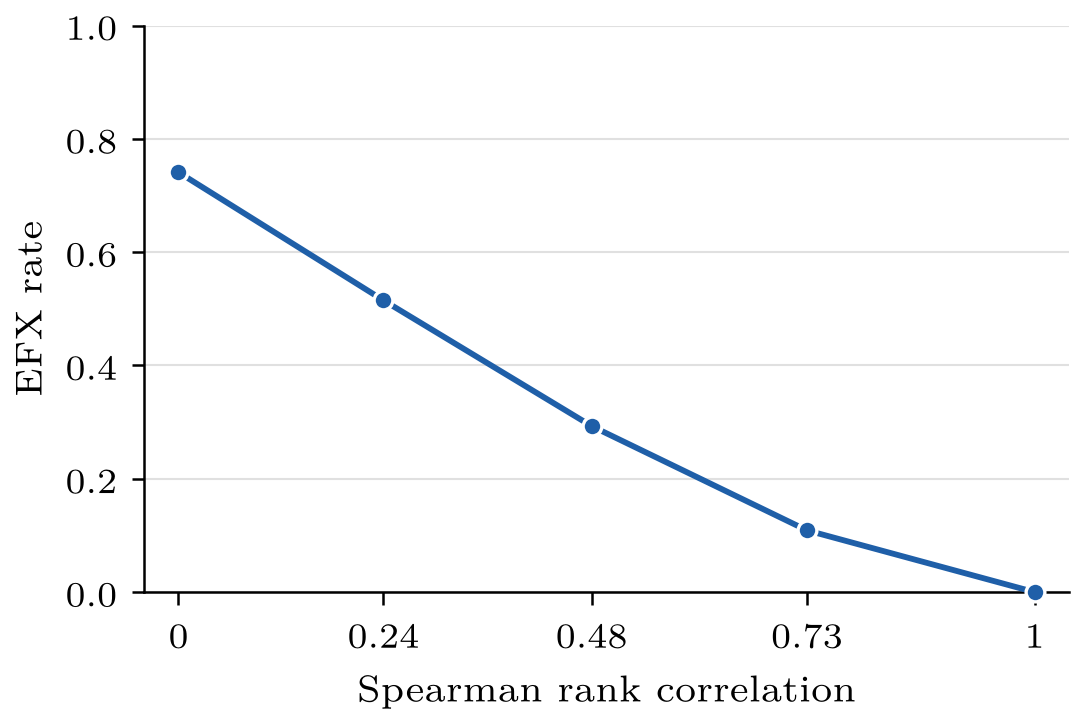
\includegraphics[width=0.6\linewidth]{agreement_rate.png}
    \caption{EFX rate of Round Robin against the Spearman rank correlation of the world from which
instances are drawn, for $n=4$ agents, $m=12$ goods and Gini $0.52$ ($\theta=1$).
Each point rests on $R=20{,}000$ instances.}
    \label{fig:placeholder}
\end{figure}


\section{Dispersion}\label{sec:dispersion}
%% FUNCTION: Shows how the EFX rate of round robin changes with the dispersion of values, all
%% other quantities at the reference levels. Round robin uses only rankings, so its allocation is
%% the same for every level of dispersion; dispersion only changes how this fixed allocation is
%% evaluated. As dispersion vanishes and the number of goods is divisible by the number of agents,
%% the EFX rate tends to one (proven, for every allocation with equal bundle sizes). Since this
%% limit depends on equal bundle sizes, the next section turns to the number of goods per agent.

\section{Bundle Size}\label{sec:bundlesize}
%% FUNCTION: Shows that round robin is guaranteed to be EFX when every agent receives at most two
%% goods and all favourite goods differ, and that this guarantee breaks as soon as one agent
%% receives three goods. Since this break coincides with a change in divisibility, the section
%% leads to the next one.

We define "collision-freeness" as follows: All agents have different favorite goods. The collision rate $1-\#\{distinct favourite goods\}/n$. For $\rho = 1$ it equals to $1-1/n$. Collision-freeness does not occur there.

$\textit{Lemma}$: 

If the instance is collision-free, only Agent $i$ can envy Agent $j$, when $|A_j|>= 3$

Proof: Withtout collision, any agents receives their favourite good in the first round. When $A_j$ only has two goods, after eleminating one good the bundle only has one good left. And that good is not more valuable than his own favourite good. $m=< 2n$ ensures $|A_j| =< 2$

Implication: If the Instance is Collision free and $m=< 2n \Rightarrow RR-Allocation is EFX$

We checked this for every cell. 336 cells with $m=<2n$ and $\rho < 1$, all six $\theta$, 1.388.388 collision free instances, 0 exceptions.

The guarantee does not need an assumption about the distribution.

bitte die tabelle hierhin anteil collsionfree instances.

This condition gets rare quickly. From a ration of 0,749 for ( n =2, rho= 0) to 0,010 for (n=5, rho = 0,75) which only are 193 of 20000 instances.


\begin{figure}
    \centering
    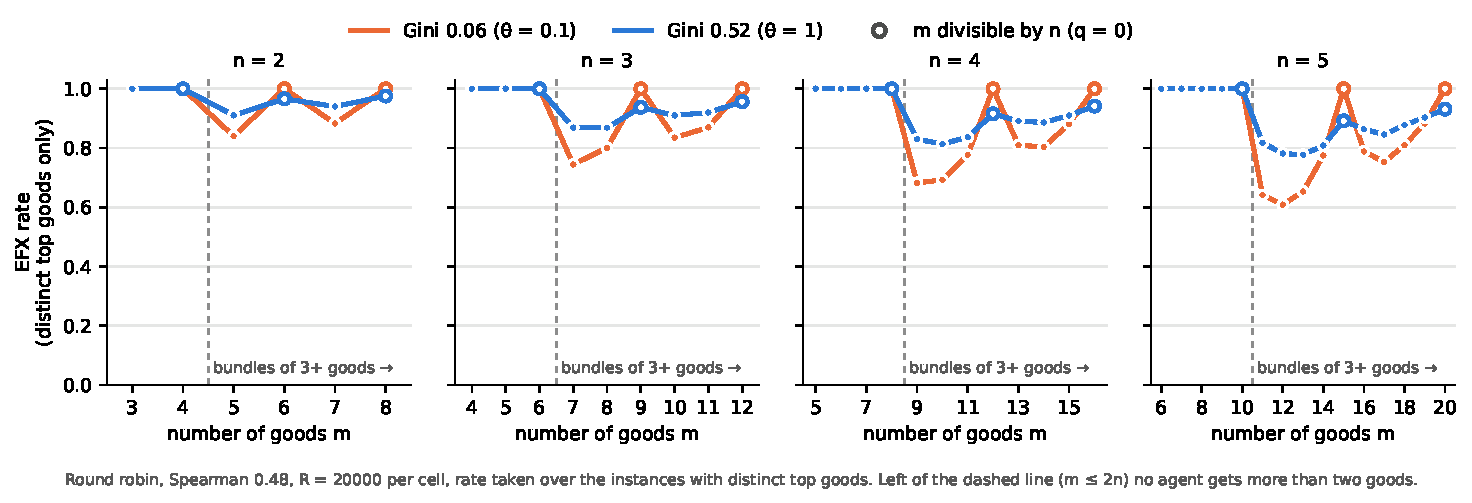
\includegraphics[width=1\linewidth]{block1_fig_break.pdf}
    \caption{Enter Caption}
    \label{fig:placeholder}
\end{figure}

For $n=4$, for $m=<8$ goods, meaning bundle size r=<2 we have a continous EFX Allocation through RR. At 9 goods, we conceive a efx bump to 0,830 (with gini 0,52) and 0,682 (at gini 0,06)
The EFX-quote under kollision free instances show a reocurring pattern that with the divisability of revover.

If we consider all instances however, those trends do not really show in the total graphic.

A bundle with two goods means for the EF1 EFX connection, lead $>=$ gap or "my bundle" $>=$ his best good. and thats secured by the own fav good. 
With three goods now its "my goods vs his two best goods" and the own fav good cannot secure both of them.
Thus, the only endangered pairs are "two vs three goods", for r=2 that are $(n-q) \cdot q$ pairs. 

With smaller $\theta$ is the EFX drop bigger, becaus the structurall lead of the pairs goes to null. 

We assume that the recovery after the drop bc of the growing lead.

Limitations, the depth of the drop also growths with $\rho$ ($n=5$: 0,942 bei $\rho=0$, 0,602 bei $\rho=0{,}75$). The graphic shows the case for $\rho = 0,75$

Another limitation is the assumption about the group we consider itself. in the real world, it rather unusual that everyone has their own favoutie good. It is rather decriptive and based on the quantitave model.

We also have to consider that the gap at 2n+1 can have two infuences.first that for the first time we have a bundle size of 3 but also the rest and divisability goes from 0 to 1. The drop could be the reslut of both changes, however you can split the two effects. becaus for smaller m<=2 there are also q>0  and the efx quote is still 1. The q alone does not break the EFX quote. But this only counts if we only consider the instances where there is collision freeness, considers for all instances this statement does not apply. 

Additionally our Lemma in independet from our distribution bc it only considers the values. If another valuation model creates values where each agents has a own favouite good, this Lemma also applies.

Our emperical foundings also allign with the scientific research, stating that Round Robin has dificouklties of finding ERX with q > 0 with cnstant proability. For an asymptotic case of our collision mechansims \cite{manurangsi2021}.

Also the EFX existance for m=<2n is proved. Moreover \cite{amanatidis2020multiple} prove that there exist and EFX alloctatin until m=<n+3






If every agent receives at most two goods and all favourite goods differ, use Round Robin: EFX is guaranteed, and both conditions can be checked in advance.“ Dazu: Die Bedingung wird mit mehr Personen und mehr Einigkeit schnell selten, und darüber hinaus bricht die Garantie.

How already consideres broadly. A central question is now how the drop behaves with other q's. 
\section{Divisibility}\label{sec:divisibility}
%% FUNCTION: Shows that whether the number of goods is divisible by the number of agents decides
%% the outcome when values are similar. With identical valuations and no divisibility round robin
%% never achieves EFX. The explanation is a structural part of the lead that exists only when all
%% bundles have equal size. The effect fades when values become very unequal, which raises the
%% question of what matters then.


\section{Number of Agents}\label{sec:agents}
%% FUNCTION: Shows that with the same number of goods per agent, EFX becomes rarer as more agents
%% take part, and separates the contribution of colliding favourite goods from the growing number
%% of agent pairs. Since the risk lies with the agents who pick last, the section asks whether a
%% different picking order helps.


\section{Round Robin, Random Allocation and Reversing the Last Round}\label{sec:random}
%% FUNCTION: Compares round robin with the balanced random benchmark that models allocating
%% somehow. With little or moderate agreement, round robin is far ahead. With full agreement and
%% a number of goods not divisible by the number of agents, round robin fails EFX with certainty
%% (proven), while random allocation fails only almost always. Reversing the last round, which is
%% just as easy to carry out by hand, removes exactly the pairs at which round robin fails there
%% (known results) and helps substantially when agents receive few goods or values are similar
%% (measured, exploratory).

% Dropped 10.11.: \section{Picking Order}\label{sec:sequences}
%% FUNCTION: Compares round robin with three simple variants of the picking order that are just as
%% easy to run by hand. It shows where they improve the EFX rate and why the largest gains come
%% from who receives the extra goods. This section is exploratory.



\chapter{Round Robin versus Random Allocation}\label{ch:random}

FUNCTION: This chapter compares round robin with allocating the goods somehow. It introduces
the balanced random allocation as a generous benchmark, shows where round robin is far ahead and
where it fails EFX systematically, and presents reversing the last round as a simple remedy that
is just as easy to carry out by hand.

\section{Balanced Random Allocation as a Generous Benchmark}\label{sec:random}
FUNCTION: Defines the balanced random allocation (same bundle sizes as round robin, values
ignored) and explains why it is a generous model of allocating without any method. Figure:
EFX rate of round robin and of random allocation against Spearman in the reference cell. With
little or moderate agreement, round robin is far ahead (measured).

\section{Where Round Robin Fails Systematically}\label{sec:random-failure}
FUNCTION: With full agreement and a number of goods not divisible by the number of agents, round
robin fails to reach EFX with certainty (proven, Section~\ref{sec:divisibility-identical}), while
random allocation fails only almost always. Wording: systematic failure to reach EFX, never
unfair, since round robin remains EF1. Figure: full agreement, $n=4$, EFX rate against $m$ for
round robin, last round reversed and random allocation.

\section{Reversing the Last Round as a Simple Remedy}\label{sec:reversed}
FUNCTION: Short and exploratory. Reversing the last round removes exactly the pairs at which
round robin fails there. The guarantees are results of other authors (Manurangsi and Suksompong
2021; Amanatidis, Markakis and Ntokos 2020). Measured: it helps substantially when agents receive
few goods or values are similar.

\chapter{Discussion}\label{ch:discussion}

FUNCTION: This chapter discusses what concerns all results jointly. Limitations of individual
results are already discussed where they arise in Chapters 4 and 5.

\section{Limitations}\label{sec:limitations}
FUNCTION: A single family of value distributions, paired rather than independent comparisons,
the existence assumption in the open region, Spearman describes the distribution and not an
instance, the generous random benchmark, the exploratory status of reversing the last round, and
the assumption that agents pick truthfully.

\section{Outlook}\label{sec:outlook}
FUNCTION: Open questions at the level of a bachelor thesis: the limit without divisibility,
whether the EFX rate stays below one for every positive dispersion beyond the smallest case,
robustness to other value distributions, and the measured patterns that remain unexplained.

\chapter{Conclusion}\label{ch:conclusion}
%% FUNCTION: Collects the recommendations of Chapters 4 and 5 in answer to the research question
%% and presents them in one decision table with a status column.

We asked how often Round Robin achieves EFX and under which conditions it is therefore a good
heuristic for EFX. Round Robin is attractive because people can carry it out by hand, and it
always guarantees EF1. It has, however, no constant guarantee for approximate EFX, so its value
as a heuristic for EFX can only be judged in the average case. We simulated $20{,}000$ instances
for each combination of two to five agents, up to four goods per agent, five levels of agreement
and six levels of dispersion, and varied one condition at a time around a reference cell with
four agents and twelve goods.

In the reference cell, Round Robin achieves EFX in $0.293$ of the instances. Whether this is a
good or a poor result depends on the conditions, and Table~\ref{tab:decision} collects them. Three
conditions favour Round Robin: little agreement among the agents, similar values together with a
number of goods divisible by the number of agents, and few goods per agent with distinct
favourite goods, where EFX is even guaranteed. Three conditions work against it: strong
agreement, strongly differing values and many agents. Under full agreement without
divisibility, Round Robin fails EFX with certainty, and reversing the order of the last round is
a remedy that is just as easy to carry out. Compared with dividing the goods somehow, Round Robin
is far ahead unless the agents agree strongly.

\begin{table}[ht]
  \centering
  \caption{When Round Robin is a good heuristic for EFX. Status: proven results hold for every
  valuation of the stated kind; measured results hold in our simulation design; exploratory
  results rest on rules fixed after individual cells were known.}
  \label{tab:decision}
  \small
  \begin{tabular}{p{4.3cm}p{5.6cm}p{2.2cm}l}
    \toprule
    Situation & Recommendation & Status & Section \\
    \midrule
    At most two goods per person, distinct favourite goods
      & Use Round Robin; EFX is guaranteed
      & proven & \ref{sec:bundlesize} \\
    Similar values, number of goods divisible
      & Round Robin or any split into equal bundle sizes is almost always EFX
      & proven (limit), measured & \ref{sec:dispersion-limit} \\
    Similar values, number of goods not divisible
      & Round Robin is better than a random split, but often narrowly misses EFX
      & measured & \ref{sec:divisibility}, \ref{sec:random} \\
    Strongly differing values
      & Divisibility no longer matters; Round Robin fails more often and more deeply
      & measured & \ref{sec:dispersion}, \ref{sec:divisibility} \\
    Little to moderate agreement
      & Use Round Robin; far better than a random split
      & measured & \ref{sec:agreement}, \ref{sec:random} \\
    Strong agreement
      & Expect Round Robin to fail more often and by more
      & measured & \ref{sec:agreement} \\
    Full agreement, number of goods not divisible
      & Never plain Round Robin; reverse the last round, which helps with few goods per person or similar values
      & proven (Round Robin), measured, exploratory (remedy) & \ref{sec:divisibility-identical}, \ref{sec:reversed} \\
    More goods per person
      & Raises the EFX rate, unless agreement is strong
      & measured, exploratory & \ref{sec:goods} \\
    More people, same goods per person
      & EFX becomes rarer; with agreement, failures also become deeper
      & measured & \ref{sec:agents} \\
    \bottomrule
  \end{tabular}
\end{table}

Our contributions are threefold. First, we measure how often Round Robin achieves EFX and how far
it misses it, for small numbers of agents and for correlated values, where existing results are
either asymptotic or concern other targets. Second, we prove three simple statements that delimit
the measurements: a guarantee for at most two goods per agent with distinct favourite goods, the
certain failure under identical valuations without divisibility, and the limit for vanishing
dispersion with equal bundle sizes. Third, we compare Round Robin with a random split and with a
reversed last round, which turns the average case results into advice for people who divide goods
by hand. All measured statements rest on one family of value distributions and, for four and five
agents, on the assumption that an EFX allocation exists (Section~\ref{sec:limitations}).


\printbibliography
\cleardoublepage

\appendix
% \chapter{Proofs}\label{app:proofs}

%% FUNCTION: Contains full proofs that would interrupt the argument in the main text.

  % no long proofs at present; all proofs are in the main text
\chapter{Full Tables}\label{app:tables}
%% FUNCTION: Reports the EFX rate of round robin for every pair (n, m) of the design, once over
%% dispersion and once over agreement, so that every cell behind the figures can be looked up.
%% Generated by Claude outputs/appB_tables.py from the confirmatory run.

Tables~\ref{tab:full-gini} and~\ref{tab:full-spearman} report the EFX rate of Round Robin for
every pair $(n,m)$ of the design, each based on $R=20{,}000$ instances. An entry of exactly $1$ or
$0$ means that all or none of the instances are EFX; $0.000$ denotes a positive rate below
$0.0005$.

\begin{table}[p]
  \centering
  \caption{EFX rate of Round Robin by dispersion, at Spearman $0.48$ ($\rho=0.5$).}
  \label{tab:full-gini}
  \footnotesize
  \begin{tabular}{rrrr cccccc}
    \toprule
    & & & & \multicolumn{6}{c}{Gini ($\theta$)} \\
    $n$ & $m$ & $r$ & $q$ & 0.06 (0.1) & 0.14 (0.25) & 0.28 (0.5) & 0.40 (0.75) & 0.52 (1) & 0.71 (1.5) \\
    \midrule
2 & 3 & 1 & 1 & 0.463 & 0.463 & 0.463 & 0.463 & 0.463 & 0.463 \\
2 & 4 & 2 & 0 & 1 & 0.982 & 0.818 & 0.701 & 0.643 & 0.588 \\
2 & 5 & 2 & 1 & 0.564 & 0.564 & 0.564 & 0.566 & 0.569 & 0.572 \\
2 & 6 & 3 & 0 & 1 & 0.982 & 0.831 & 0.735 & 0.687 & 0.645 \\
2 & 7 & 3 & 1 & 0.693 & 0.688 & 0.680 & 0.676 & 0.671 & 0.664 \\
2 & 8 & 4 & 0 & 1 & 0.989 & 0.875 & 0.792 & 0.750 & 0.710 \\
\midrule
3 & 4 & 1 & 1 & 0.250 & 0.250 & 0.250 & 0.250 & 0.250 & 0.250 \\
3 & 5 & 1 & 2 & 0.322 & 0.320 & 0.287 & 0.259 & 0.243 & 0.227 \\
3 & 6 & 2 & 0 & 1 & 0.965 & 0.645 & 0.463 & 0.379 & 0.310 \\
3 & 7 & 2 & 1 & 0.381 & 0.382 & 0.362 & 0.339 & 0.323 & 0.306 \\
3 & 8 & 2 & 2 & 0.457 & 0.449 & 0.403 & 0.368 & 0.348 & 0.335 \\
3 & 9 & 3 & 0 & 1 & 0.971 & 0.696 & 0.533 & 0.459 & 0.397 \\
3 & 10 & 3 & 1 & 0.570 & 0.561 & 0.518 & 0.471 & 0.446 & 0.415 \\
3 & 11 & 3 & 2 & 0.626 & 0.612 & 0.556 & 0.507 & 0.477 & 0.445 \\
3 & 12 & 4 & 0 & 1 & 0.982 & 0.772 & 0.625 & 0.551 & 0.482 \\
\midrule
4 & 5 & 1 & 1 & 0.150 & 0.150 & 0.150 & 0.150 & 0.150 & 0.150 \\
4 & 6 & 1 & 2 & 0.122 & 0.122 & 0.114 & 0.105 & 0.100 & 0.095 \\
4 & 7 & 1 & 3 & 0.248 & 0.245 & 0.189 & 0.145 & 0.124 & 0.106 \\
4 & 8 & 2 & 0 & 1 & 0.952 & 0.505 & 0.289 & 0.212 & 0.155 \\
4 & 9 & 2 & 1 & 0.288 & 0.290 & 0.249 & 0.205 & 0.179 & 0.157 \\
4 & 10 & 2 & 2 & 0.252 & 0.247 & 0.222 & 0.198 & 0.182 & 0.168 \\
4 & 11 & 2 & 3 & 0.393 & 0.384 & 0.304 & 0.246 & 0.215 & 0.190 \\
4 & 12 & 3 & 0 & 1 & 0.959 & 0.574 & 0.375 & 0.293 & 0.230 \\
4 & 13 & 3 & 1 & 0.499 & 0.491 & 0.412 & 0.339 & 0.298 & 0.254 \\
4 & 14 & 3 & 2 & 0.466 & 0.448 & 0.395 & 0.342 & 0.307 & 0.270 \\
4 & 15 & 3 & 3 & 0.605 & 0.583 & 0.475 & 0.392 & 0.342 & 0.291 \\
4 & 16 & 4 & 0 & 1 & 0.977 & 0.693 & 0.506 & 0.409 & 0.329 \\
\midrule
5 & 6 & 1 & 1 & 0.095 & 0.095 & 0.095 & 0.095 & 0.095 & 0.095 \\
5 & 7 & 1 & 2 & 0.055 & 0.055 & 0.052 & 0.049 & 0.048 & 0.046 \\
5 & 8 & 1 & 3 & 0.079 & 0.079 & 0.067 & 0.055 & 0.049 & 0.044 \\
5 & 9 & 1 & 4 & 0.205 & 0.201 & 0.131 & 0.085 & 0.064 & 0.048 \\
5 & 10 & 2 & 0 & 1 & 0.935 & 0.395 & 0.186 & 0.119 & 0.077 \\
5 & 11 & 2 & 1 & 0.224 & 0.226 & 0.173 & 0.126 & 0.100 & 0.080 \\
5 & 12 & 2 & 2 & 0.159 & 0.155 & 0.134 & 0.111 & 0.097 & 0.082 \\
5 & 13 & 2 & 3 & 0.197 & 0.192 & 0.154 & 0.126 & 0.109 & 0.094 \\
5 & 14 & 2 & 4 & 0.373 & 0.357 & 0.242 & 0.171 & 0.138 & 0.111 \\
5 & 15 & 3 & 0 & 1 & 0.953 & 0.480 & 0.268 & 0.188 & 0.133 \\
5 & 16 & 3 & 1 & 0.453 & 0.444 & 0.339 & 0.245 & 0.193 & 0.149 \\
5 & 17 & 3 & 2 & 0.372 & 0.357 & 0.298 & 0.236 & 0.201 & 0.161 \\
5 & 18 & 3 & 3 & 0.426 & 0.401 & 0.324 & 0.259 & 0.219 & 0.176 \\
5 & 19 & 3 & 4 & 0.592 & 0.563 & 0.414 & 0.310 & 0.251 & 0.193 \\
5 & 20 & 4 & 0 & 1 & 0.973 & 0.626 & 0.402 & 0.301 & 0.218 \\
    \bottomrule
  \end{tabular}
\end{table}

\begin{table}[p]
  \centering
  \caption{EFX rate of Round Robin by agreement, at Gini $0.52$ ($\theta=1$).}
  \label{tab:full-spearman}
  \footnotesize
  \begin{tabular}{rrrr ccccc}
    \toprule
    & & & & \multicolumn{5}{c}{Spearman ($\rho$)} \\
    $n$ & $m$ & $r$ & $q$ & 0 (0) & 0.24 (0.25) & 0.48 (0.5) & 0.73 (0.75) & 1 (1) \\
    \midrule
2 & 3 & 1 & 1 & 0.667 & 0.569 & 0.463 & 0.328 & 0 \\
2 & 4 & 2 & 0 & 0.830 & 0.745 & 0.643 & 0.501 & 0.238 \\
2 & 5 & 2 & 1 & 0.802 & 0.695 & 0.569 & 0.391 & 0 \\
2 & 6 & 3 & 0 & 0.885 & 0.804 & 0.687 & 0.506 & 0.069 \\
2 & 7 & 3 & 1 & 0.888 & 0.802 & 0.671 & 0.465 & 0 \\
2 & 8 & 4 & 0 & 0.930 & 0.859 & 0.750 & 0.555 & 0.021 \\
\midrule
3 & 4 & 1 & 1 & 0.496 & 0.371 & 0.250 & 0.129 & 0 \\
3 & 5 & 1 & 2 & 0.519 & 0.373 & 0.243 & 0.119 & 0 \\
3 & 6 & 2 & 0 & 0.688 & 0.533 & 0.379 & 0.224 & 0.049 \\
3 & 7 & 2 & 1 & 0.666 & 0.494 & 0.323 & 0.153 & 0 \\
3 & 8 & 2 & 2 & 0.708 & 0.534 & 0.348 & 0.161 & 0 \\
3 & 9 & 3 & 0 & 0.804 & 0.640 & 0.459 & 0.240 & 0.004 \\
3 & 10 & 3 & 1 & 0.808 & 0.643 & 0.446 & 0.214 & 0 \\
3 & 11 & 3 & 2 & 0.835 & 0.678 & 0.477 & 0.236 & 0 \\
3 & 12 & 4 & 0 & 0.888 & 0.748 & 0.551 & 0.296 & 0.000 \\
\midrule
4 & 5 & 1 & 1 & 0.399 & 0.262 & 0.150 & 0.056 & 0 \\
4 & 6 & 1 & 2 & 0.354 & 0.203 & 0.100 & 0.034 & 0 \\
4 & 7 & 1 & 3 & 0.424 & 0.251 & 0.124 & 0.045 & 0 \\
4 & 8 & 2 & 0 & 0.577 & 0.374 & 0.212 & 0.093 & 0.010 \\
4 & 9 & 2 & 1 & 0.562 & 0.347 & 0.179 & 0.058 & 0 \\
4 & 10 & 2 & 2 & 0.581 & 0.362 & 0.182 & 0.056 & 0 \\
4 & 11 & 2 & 3 & 0.643 & 0.411 & 0.215 & 0.069 & 0 \\
4 & 12 & 3 & 0 & 0.741 & 0.515 & 0.293 & 0.109 & 0.000 \\
4 & 13 & 3 & 1 & 0.751 & 0.522 & 0.298 & 0.098 & 0 \\
4 & 14 & 3 & 2 & 0.772 & 0.542 & 0.307 & 0.098 & 0 \\
4 & 15 & 3 & 3 & 0.807 & 0.588 & 0.342 & 0.116 & 0 \\
4 & 16 & 4 & 0 & 0.856 & 0.661 & 0.409 & 0.159 & 0 \\
\midrule
5 & 6 & 1 & 1 & 0.332 & 0.191 & 0.095 & 0.028 & 0 \\
5 & 7 & 1 & 2 & 0.267 & 0.123 & 0.048 & 0.012 & 0 \\
5 & 8 & 1 & 3 & 0.272 & 0.123 & 0.049 & 0.011 & 0 \\
5 & 9 & 1 & 4 & 0.355 & 0.161 & 0.064 & 0.018 & 0 \\
5 & 10 & 2 & 0 & 0.491 & 0.265 & 0.119 & 0.035 & 0.002 \\
5 & 11 & 2 & 1 & 0.482 & 0.246 & 0.100 & 0.021 & 0 \\
5 & 12 & 2 & 2 & 0.500 & 0.254 & 0.097 & 0.019 & 0 \\
5 & 13 & 2 & 3 & 0.531 & 0.276 & 0.109 & 0.022 & 0 \\
5 & 14 & 2 & 4 & 0.600 & 0.331 & 0.138 & 0.029 & 0 \\
5 & 15 & 3 & 0 & 0.690 & 0.412 & 0.188 & 0.047 & 0 \\
5 & 16 & 3 & 1 & 0.705 & 0.435 & 0.193 & 0.042 & 0 \\
5 & 17 & 3 & 2 & 0.721 & 0.443 & 0.201 & 0.044 & 0 \\
5 & 18 & 3 & 3 & 0.755 & 0.471 & 0.219 & 0.047 & 0 \\
5 & 19 & 3 & 4 & 0.788 & 0.519 & 0.251 & 0.056 & 0 \\
5 & 20 & 4 & 0 & 0.831 & 0.581 & 0.301 & 0.084 & 0 \\
    \bottomrule
  \end{tabular}
\end{table}

% \chapter{Lead versus Gap}\label{sec:leadgap}

FUNCTION: Reads the known argument that round robin is EF1 (Section~\ref{sec:rrEF1}) as a lead
that is never negative. EFX holds exactly when this lead covers a gap between two single goods.
The lead grows with every round, the gap does not; a structural part of the lead exists only when
all bundles have equal size. Moved here from Chapter 2 on 10.11.; may return to the main text.
  % Lead versus Gap: kept out for now (decision 10.11.)

\backmatter
% Declaration, \input from main.tex
\chapter*{Declaration}
Ich  versichere  wahrheitsgemäß,  die  Arbeit selbstständig  verfasst,  alle  benutzten  Hilfsmittel  voll\-ständig  und  genau  angegeben  und  alles kenntlich  gemacht  zu  haben,  was  aus  Arbeiten  anderer  unverändert  oder  mit  Abänderungen entnommen  wurde  sowie die Satzung  des  KIT  zur  Sicherung guter wissenschaftlicher Praxis in der jeweils gültigen Fassung beachtet zu haben.\\ \\
\noindent Karlsruhe,  xx/xx/xxxx
\\ \\ \\ \\
------------------------------------\\
Francisco Waggershauser


\addcontentsline{toc}{chapter}{Declaration on Proper Scientific Conduct} % Eintrag zum Inhaltsverzeichnis hinzufügen/add entry to table of contents


\end{document}
